\documentclass[10pt,a4paper,onecolumn]{article}
\usepackage{marginnote}
\usepackage{graphicx}
\usepackage{xcolor}
\usepackage{authblk,etoolbox}
\usepackage{titlesec}
\usepackage{calc}
\usepackage{tikz}
\usepackage{hyperref}
\hypersetup{colorlinks,breaklinks,
            urlcolor=[rgb]{0.0, 0.5, 1.0},
            linkcolor=[rgb]{0.0, 0.5, 1.0}}
\usepackage{caption}
\usepackage{tcolorbox}
\usepackage{amssymb,amsmath}
\usepackage{ifxetex,ifluatex}
\usepackage{seqsplit}
\usepackage{fixltx2e} % provides \textsubscript
\usepackage[
  backend=biber,
%  style=alphabetic,
%  citestyle=numeric
]{biblatex}
\bibliography{paper.bib}



% --- Page layout -------------------------------------------------------------
\usepackage[top=3.5cm, bottom=3cm, right=1.5cm, left=1.0cm,
            headheight=2.2cm, reversemp, includemp, marginparwidth=4.5cm]{geometry}

% --- Default font ------------------------------------------------------------
% \renewcommand\familydefault{\sfdefault}

% --- Style -------------------------------------------------------------------
\renewcommand{\bibfont}{\small \sffamily}
\renewcommand{\captionfont}{\small\sffamily}
\renewcommand{\captionlabelfont}{\bfseries}

% --- Section/SubSection/SubSubSection ----------------------------------------
\titleformat{\section}
  {\normalfont\sffamily\Large\bfseries}
  {}{0pt}{}
\titleformat{\subsection}
  {\normalfont\sffamily\large\bfseries}
  {}{0pt}{}
\titleformat{\subsubsection}
  {\normalfont\sffamily\bfseries}
  {}{0pt}{}
\titleformat*{\paragraph}
  {\sffamily\normalsize}


% --- Header / Footer ---------------------------------------------------------
\usepackage{fancyhdr}
\pagestyle{fancy}
\fancyhf{}
%\renewcommand{\headrulewidth}{0.50pt}
\renewcommand{\headrulewidth}{0pt}
\fancyhead[L]{\hspace{-0.75cm}\includegraphics[width=5.5cm]{C:/Users/ben29/AppData/Local/R/win-library/4.4/rticles/rmarkdown/templates/joss/resources/JOSS-logo.png}}
\fancyhead[C]{}
\fancyhead[R]{}
\renewcommand{\footrulewidth}{0.25pt}

\fancyfoot[L]{\footnotesize{\sffamily , (). fairmetrics: An R package
for group fairness
evaluation. \textit{Journal of Open Source Software}, (), . \href{https://doi.org/}{https://doi.org/}}}


\fancyfoot[R]{\sffamily \thepage}
\makeatletter
\let\ps@plain\ps@fancy
\fancyheadoffset[L]{4.5cm}
\fancyfootoffset[L]{4.5cm}

% --- Macros ---------

\definecolor{linky}{rgb}{0.0, 0.5, 1.0}

\newtcolorbox{repobox}
   {colback=red, colframe=red!75!black,
     boxrule=0.5pt, arc=2pt, left=6pt, right=6pt, top=3pt, bottom=3pt}

\newcommand{\ExternalLink}{%
   \tikz[x=1.2ex, y=1.2ex, baseline=-0.05ex]{%
       \begin{scope}[x=1ex, y=1ex]
           \clip (-0.1,-0.1)
               --++ (-0, 1.2)
               --++ (0.6, 0)
               --++ (0, -0.6)
               --++ (0.6, 0)
               --++ (0, -1);
           \path[draw,
               line width = 0.5,
               rounded corners=0.5]
               (0,0) rectangle (1,1);
       \end{scope}
       \path[draw, line width = 0.5] (0.5, 0.5)
           -- (1, 1);
       \path[draw, line width = 0.5] (0.6, 1)
           -- (1, 1) -- (1, 0.6);
       }
   }

% --- Title / Authors ---------------------------------------------------------
% patch \maketitle so that it doesn't center
\patchcmd{\@maketitle}{center}{flushleft}{}{}
\patchcmd{\@maketitle}{center}{flushleft}{}{}
% patch \maketitle so that the font size for the title is normal
\patchcmd{\@maketitle}{\LARGE}{\LARGE\sffamily}{}{}
% patch the patch by authblk so that the author block is flush left
\def\maketitle{{%
  \renewenvironment{tabular}[2][]
    {\begin{flushleft}}
    {\end{flushleft}}
  \AB@maketitle}}
\makeatletter
\renewcommand\AB@affilsepx{ \protect\Affilfont}
%\renewcommand\AB@affilnote[1]{{\bfseries #1}\hspace{2pt}}
\renewcommand\AB@affilnote[1]{{\bfseries #1}\hspace{3pt}}
\makeatother
\renewcommand\Authfont{\sffamily\bfseries}
\renewcommand\Affilfont{\sffamily\small\mdseries}
\setlength{\affilsep}{1em}


\ifnum 0\ifxetex 1\fi\ifluatex 1\fi=0 % if pdftex
  \usepackage[T1]{fontenc}
  \usepackage[utf8]{inputenc}

\else % if luatex or xelatex
  \ifxetex
    \usepackage{mathspec}
  \else
    \usepackage{fontspec}
  \fi
  \defaultfontfeatures{Ligatures=TeX,Scale=MatchLowercase}

\fi
% use upquote if available, for straight quotes in verbatim environments
\IfFileExists{upquote.sty}{\usepackage{upquote}}{}
% use microtype if available
\IfFileExists{microtype.sty}{%
\usepackage{microtype}
\UseMicrotypeSet[protrusion]{basicmath} % disable protrusion for tt fonts
}{}

\usepackage{hyperref}
\hypersetup{unicode=true,
            pdftitle={fairmetrics: An R package for group fairness evaluation},
            pdfborder={0 0 0},
            breaklinks=true}
\urlstyle{same}  % don't use monospace font for urls
\usepackage{graphicx,grffile}
\makeatletter
\newsavebox\pandoc@box
\newcommand*\pandocbounded[1]{% scales image to fit in text height/width
  \sbox\pandoc@box{#1}%
  \Gscale@div\@tempa{\textheight}{\dimexpr\ht\pandoc@box+\dp\pandoc@box\relax}%
  \Gscale@div\@tempb{\linewidth}{\wd\pandoc@box}%
  \ifdim\@tempb\p@<\@tempa\p@\let\@tempa\@tempb\fi% select the smaller of both
  \ifdim\@tempa\p@<\p@\scalebox{\@tempa}{\usebox\pandoc@box}%
  \else\usebox{\pandoc@box}%
  \fi%
}
\makeatother
\IfFileExists{parskip.sty}{%
\usepackage{parskip}
}{% else
\setlength{\parindent}{0pt}
\setlength{\parskip}{6pt plus 2pt minus 1pt}
}
\setlength{\emergencystretch}{3em}  % prevent overfull lines
\setcounter{secnumdepth}{0}
% Redefines (sub)paragraphs to behave more like sections
\ifx\paragraph\undefined\else
\let\oldparagraph\paragraph
\renewcommand{\paragraph}[1]{\oldparagraph{#1}\mbox{}}
\fi
\ifx\subparagraph\undefined\else
\let\oldsubparagraph\subparagraph
\renewcommand{\subparagraph}[1]{\oldsubparagraph{#1}\mbox{}}
\fi

% Pandoc syntax highlighting
\usepackage{color}
\usepackage{fancyvrb}
\newcommand{\VerbBar}{|}
\newcommand{\VERB}{\Verb[commandchars=\\\{\}]}
\DefineVerbatimEnvironment{Highlighting}{Verbatim}{commandchars=\\\{\}}
% Add ',fontsize=\small' for more characters per line
\usepackage{framed}
\definecolor{shadecolor}{RGB}{248,248,248}
\newenvironment{Shaded}{\begin{snugshade}}{\end{snugshade}}
\newcommand{\AlertTok}[1]{\textcolor[rgb]{0.94,0.16,0.16}{#1}}
\newcommand{\AnnotationTok}[1]{\textcolor[rgb]{0.56,0.35,0.01}{\textbf{\textit{#1}}}}
\newcommand{\AttributeTok}[1]{\textcolor[rgb]{0.13,0.29,0.53}{#1}}
\newcommand{\BaseNTok}[1]{\textcolor[rgb]{0.00,0.00,0.81}{#1}}
\newcommand{\BuiltInTok}[1]{#1}
\newcommand{\CharTok}[1]{\textcolor[rgb]{0.31,0.60,0.02}{#1}}
\newcommand{\CommentTok}[1]{\textcolor[rgb]{0.56,0.35,0.01}{\textit{#1}}}
\newcommand{\CommentVarTok}[1]{\textcolor[rgb]{0.56,0.35,0.01}{\textbf{\textit{#1}}}}
\newcommand{\ConstantTok}[1]{\textcolor[rgb]{0.56,0.35,0.01}{#1}}
\newcommand{\ControlFlowTok}[1]{\textcolor[rgb]{0.13,0.29,0.53}{\textbf{#1}}}
\newcommand{\DataTypeTok}[1]{\textcolor[rgb]{0.13,0.29,0.53}{#1}}
\newcommand{\DecValTok}[1]{\textcolor[rgb]{0.00,0.00,0.81}{#1}}
\newcommand{\DocumentationTok}[1]{\textcolor[rgb]{0.56,0.35,0.01}{\textbf{\textit{#1}}}}
\newcommand{\ErrorTok}[1]{\textcolor[rgb]{0.64,0.00,0.00}{\textbf{#1}}}
\newcommand{\ExtensionTok}[1]{#1}
\newcommand{\FloatTok}[1]{\textcolor[rgb]{0.00,0.00,0.81}{#1}}
\newcommand{\FunctionTok}[1]{\textcolor[rgb]{0.13,0.29,0.53}{\textbf{#1}}}
\newcommand{\ImportTok}[1]{#1}
\newcommand{\InformationTok}[1]{\textcolor[rgb]{0.56,0.35,0.01}{\textbf{\textit{#1}}}}
\newcommand{\KeywordTok}[1]{\textcolor[rgb]{0.13,0.29,0.53}{\textbf{#1}}}
\newcommand{\NormalTok}[1]{#1}
\newcommand{\OperatorTok}[1]{\textcolor[rgb]{0.81,0.36,0.00}{\textbf{#1}}}
\newcommand{\OtherTok}[1]{\textcolor[rgb]{0.56,0.35,0.01}{#1}}
\newcommand{\PreprocessorTok}[1]{\textcolor[rgb]{0.56,0.35,0.01}{\textit{#1}}}
\newcommand{\RegionMarkerTok}[1]{#1}
\newcommand{\SpecialCharTok}[1]{\textcolor[rgb]{0.81,0.36,0.00}{\textbf{#1}}}
\newcommand{\SpecialStringTok}[1]{\textcolor[rgb]{0.31,0.60,0.02}{#1}}
\newcommand{\StringTok}[1]{\textcolor[rgb]{0.31,0.60,0.02}{#1}}
\newcommand{\VariableTok}[1]{\textcolor[rgb]{0.00,0.00,0.00}{#1}}
\newcommand{\VerbatimStringTok}[1]{\textcolor[rgb]{0.31,0.60,0.02}{#1}}
\newcommand{\WarningTok}[1]{\textcolor[rgb]{0.56,0.35,0.01}{\textbf{\textit{#1}}}}

% tightlist command for lists without linebreak
\providecommand{\tightlist}{%
  \setlength{\itemsep}{0pt}\setlength{\parskip}{0pt}}


% Pandoc citation processing
%From Pandoc 3.1.8
% definitions for citeproc citations
\NewDocumentCommand\citeproctext{}{}
\NewDocumentCommand\citeproc{mm}{%
  \begingroup\def\citeproctext{#2}\cite{#1}\endgroup}
\makeatletter
 % allow citations to break across lines
 \let\@cite@ofmt\@firstofone
 % avoid brackets around text for \cite:
 \def\@biblabel#1{}
 \def\@cite#1#2{{#1\if@tempswa , #2\fi}}
\makeatother
\newlength{\cslhangindent}
\setlength{\cslhangindent}{1.5em}
\newlength{\csllabelwidth}
\setlength{\csllabelwidth}{3em}
\newenvironment{CSLReferences}[2] % #1 hanging-indent, #2 entry-spacing
 {\begin{list}{}{%
  \setlength{\itemindent}{0pt}
  \setlength{\leftmargin}{0pt}
  \setlength{\parsep}{0pt}
  % turn on hanging indent if param 1 is 1
  \ifodd #1
   \setlength{\leftmargin}{\cslhangindent}
   \setlength{\itemindent}{-1\cslhangindent}
  \fi
  % set entry spacing
  \setlength{\itemsep}{#2\baselineskip}}}
 {\end{list}}
\usepackage{calc}
\newcommand{\CSLBlock}[1]{#1\hfill\break}
\newcommand{\CSLLeftMargin}[1]{\parbox[t]{\csllabelwidth}{#1}}
\newcommand{\CSLRightInline}[1]{\parbox[t]{\linewidth - \csllabelwidth}{#1}\break}
\newcommand{\CSLIndent}[1]{\hspace{\cslhangindent}#1}



\title{fairmetrics: An R package for group fairness evaluation}

        \author[1]{Benjamin Smith}
          \author[1]{Jianhui Gao}
          \author[1]{Benson Chou}
          \author[1]{Jessica Gronsbell}
    
      \affil[1]{Department of Statistical Science, University of
Toronto}
  \date{\vspace{-5ex}}

\begin{document}
\maketitle

\marginpar{
  %\hrule
  \sffamily\small

  {\bfseries DOI:} \href{https://doi.org/}{\color{linky}{}}

  \vspace{2mm}

  {\bfseries Software}
  \begin{itemize}
    \setlength\itemsep{0em}
    \item \href{}{\color{linky}{Review}} \ExternalLink
    \item \href{}{\color{linky}{Repository}} \ExternalLink
    \item \href{}{\color{linky}{Archive}} \ExternalLink
  \end{itemize}

  \vspace{2mm}

  {\bfseries Submitted:} \\
  {\bfseries Published:} 

  \vspace{2mm}
  {\bfseries License}\\
  Authors of papers retain copyright and release the work under a Creative Commons Attribution 4.0 International License (\href{http://creativecommons.org/licenses/by/4.0/}{\color{linky}{CC-BY}}).
}

\section{Summary}\label{summary}

Fairness is a growing area of machine learning (ML) that focuses on
ensuring that models do not produce systematically biased outcomes
across groups defined by protected attributes, such as race, gender, or
age. The \texttt{fairmetrics} R package provides a user-friendly
framework for rigorously evaluating group-based fairness criteria,
including independence (e.g., statistical parity), separation (e.g.,
equalized odds), and sufficiency (e.g., predictive parity) for binary
protected attributes. The package provides both point and interval
estimates for a variety of commonly used criteria. \texttt{fairmetrics}
also includes an example dataset derived from the Medical Information
Mart for Intensive Care, version II (MIMIC-II) database (Goldberger et
al. 2000; J. Raffa 2016) to demonstrate its use.

\section{Statement of Need}\label{statement-of-need}

ML models are increasingly used in high-stakes domains such as criminal
justice, healthcare, finance, employment, and education (Mehrabi et al.
2021; Mattu 2016; Gao et al. 2024). Existing fairness evaluation
software report point estimates and/or visualizations, without any
measures of uncertainty. This limits users' ability to determine whether
observed disparities are statistically significant. \texttt{fairmetrics}
addresses this limitation by including confidence intervals for both
difference and ratio based fairness metrics to enable more robust and
statistically grounded fairness assessments.

\section{Fairness Criteria}\label{fairness-criteria}

\texttt{fairmetrics} is designed to evaluate fairness of binary
classification models across binary protected attributes. The package
supports the evaluation of metrics belonging to three major group
fairness criteria:

\begin{itemize}
\item
  \textbf{Independence:} Statistical Parity (compares the overall rate
  of positive predictions between groups).
\item
  \textbf{Separation:} Equal Opportunity (compares false negative rates
  between groups), Predictive Equality (compares false positive rates
  between groups), Balance for Positive Class (compares the average
  predicted probabilities among individuals whose true outcome is
  positive across groups), and Balance for Negative Class (compares the
  average predicted probabilities among individuals whose true outcome
  is negative across groups).
\item
  \textbf{Sufficiency:} Positive Predictive Parity (compares the
  positive predictive values across groups), Negative Predictive Parity
  (compares the negative predictive values across groups).
\end{itemize}

The package also includes additional metrics, such as the Brier Score
Parity (compares the Brier score across groups), Accuracy Parity
(compares the overall accuracy across groups), and Treatment Equality
(compares the ratio of false negatives to false positives across
groups).

\section{Evaluating Fairness
Criteria}\label{evaluating-fairness-criteria}

The input required to evaluate model fairness with the
\texttt{fairmetrics} package is a \texttt{data.frame} or \texttt{tibble}
containing the model's predicted probabilities, the true outcomes, and
the protected attribute. \hyperref[workflow]{Figure ~\ref*{workflow}}
shows the workflow for using \texttt{fairmetrics}.

\begin{figure}
\centering
\pandocbounded{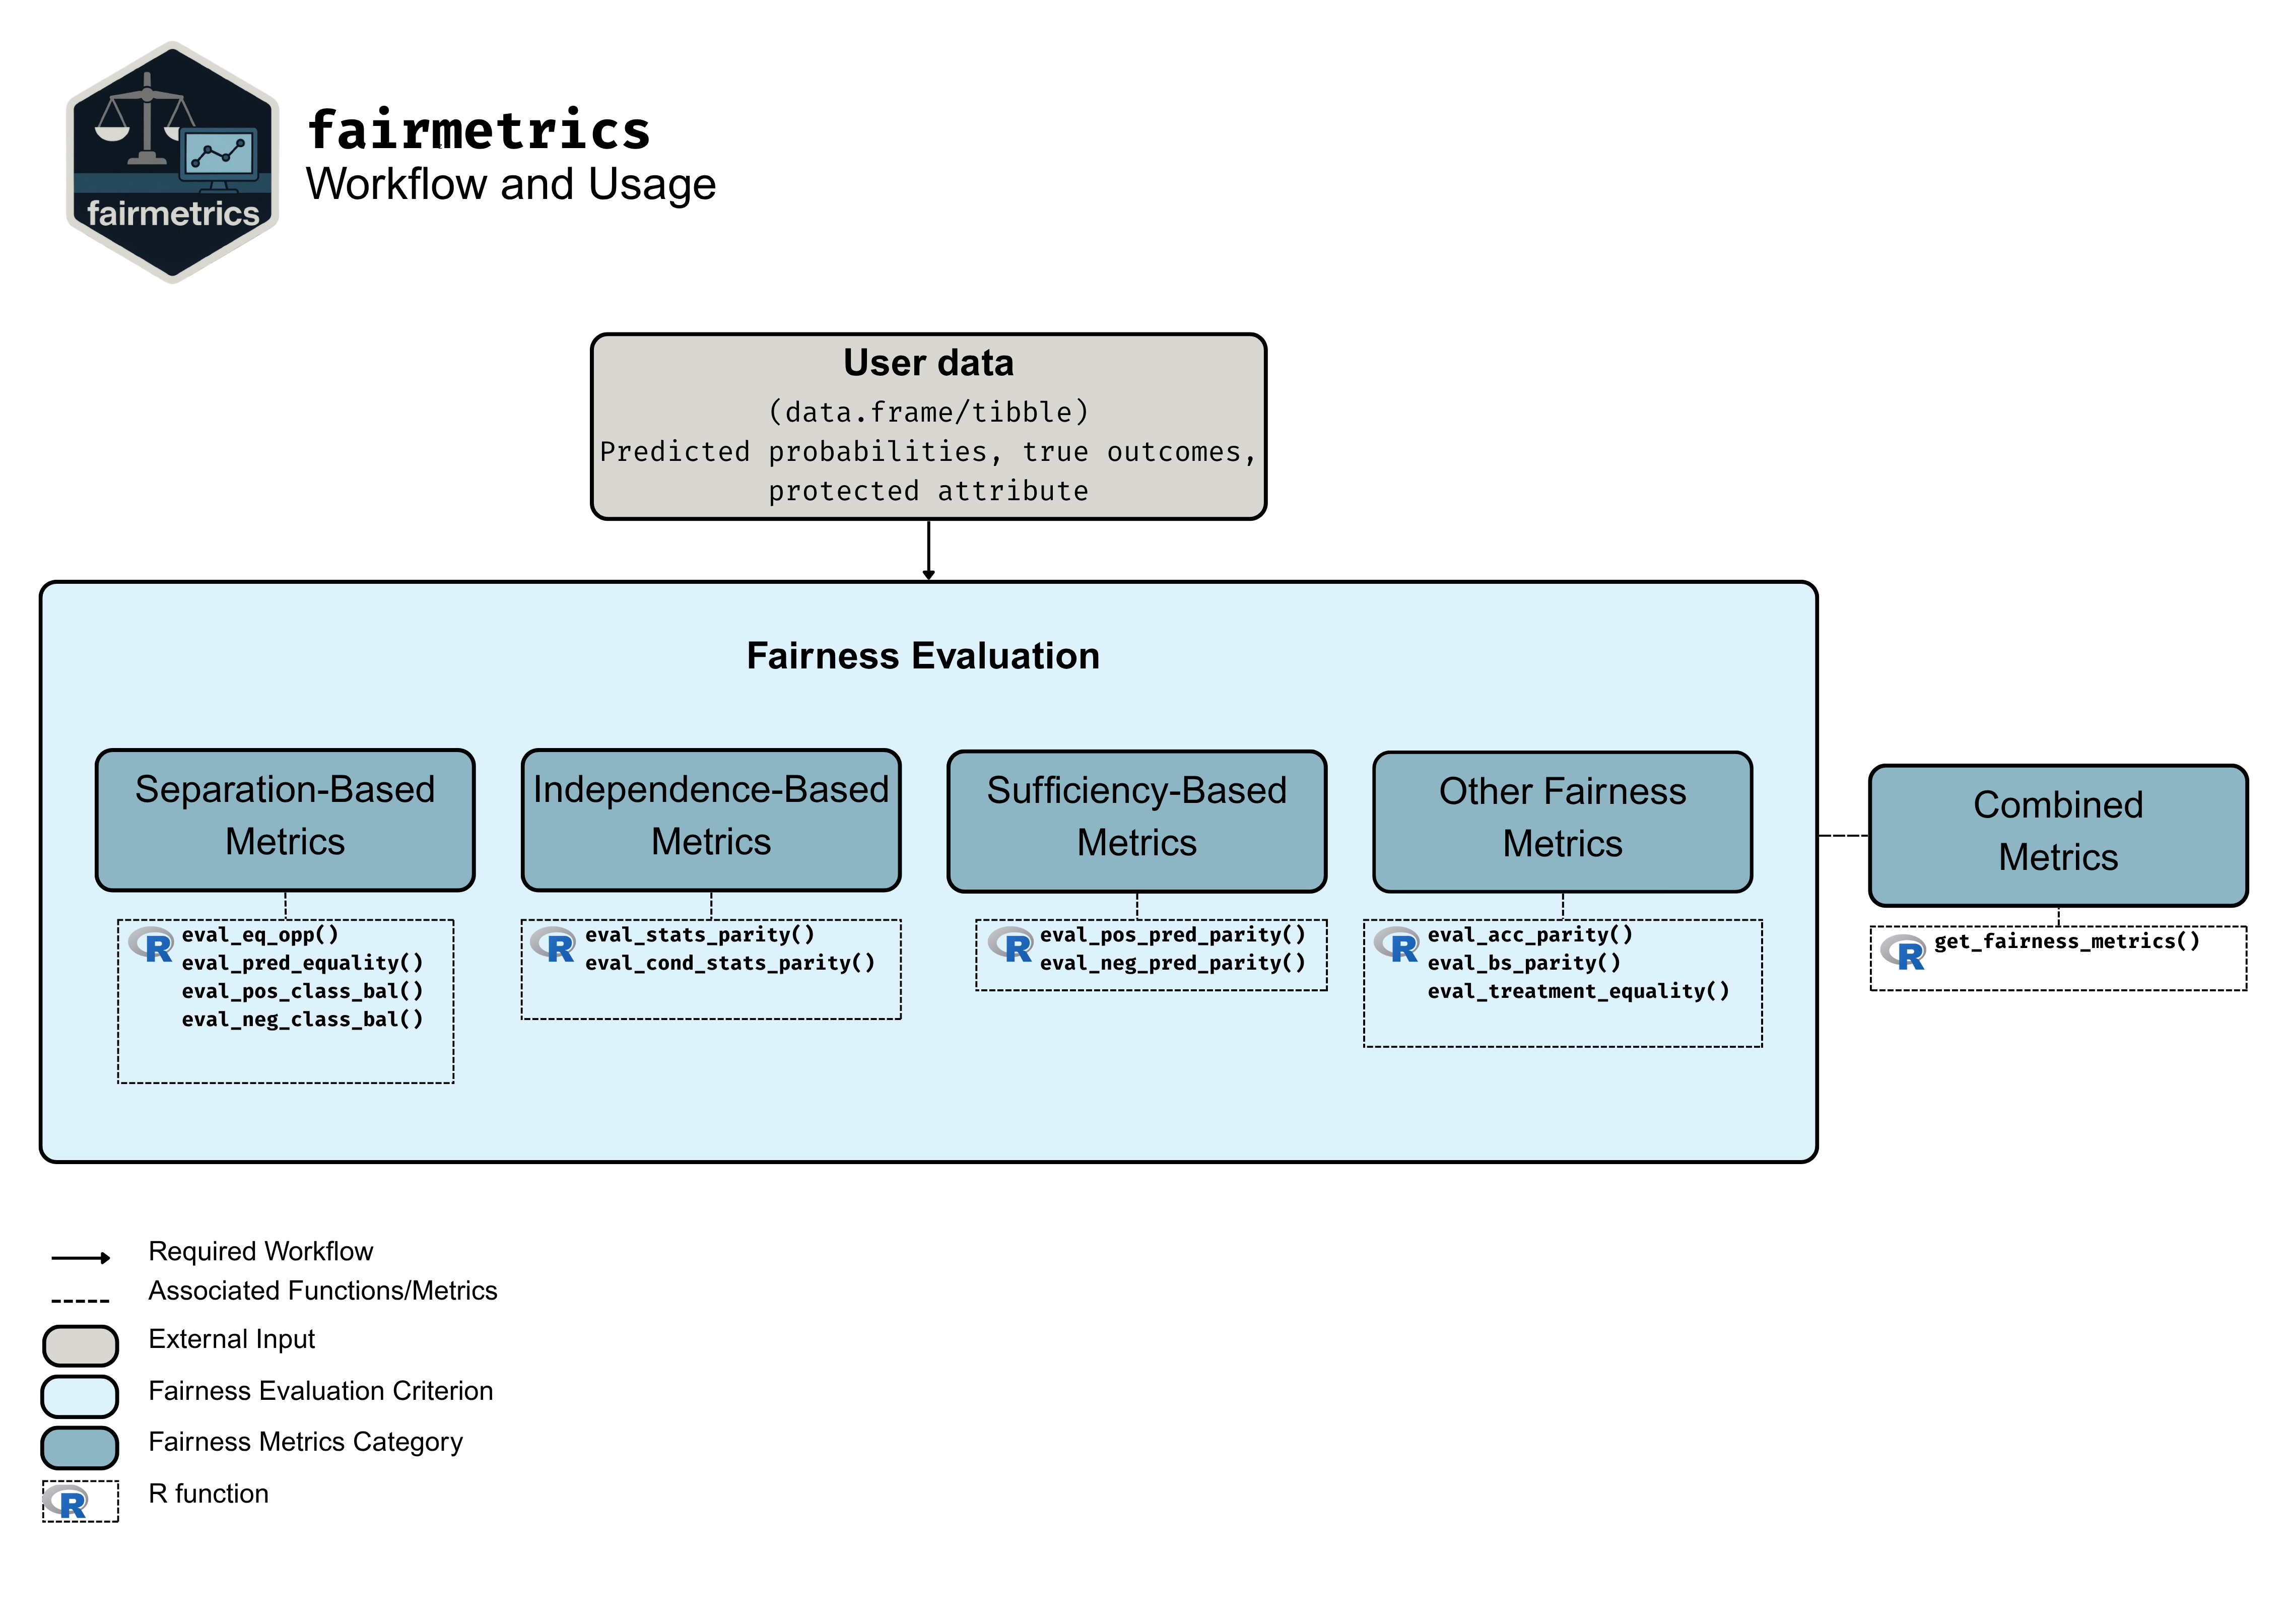
\includegraphics[keepaspectratio]{fairmetrics-workflow.png}}
\caption{Workflow for using \texttt{fairmetrics} to evaluate model
fairness across multiple criteria. \label{workflow}}
\end{figure}

A simple example of how to use the \texttt{fairmetrics} package is
illustrated below. The example makes use of the
\texttt{mimic\_preprocessed} dataset, a pre-processed version of the
Indwelling Arterial Catheter (IAC) Clinical dataset, from the MIMIC-II
clinical database (Goldberger et al. 2000; J. Raffa 2016; J. D. Raffa et
al. 2016).

While the choice of fairness metric used is context dependent, we show
all criteria available with the \texttt{get\_fairness\_metrics()}
function for illustrative purposes. In this example, we evaluate the
model's fairness with respect to the binary protected attribute
\texttt{gender}. The model is trained on a subset of the data and the
predictions are made and evaluated on a test set. A statistically
significant difference across groups at a given level of significance is
indicated when the confidence interval for a difference-based metric
does not include zero or when the interval for a ratio-based metric does
not include one.

\begin{Shaded}
\begin{Highlighting}[]
\CommentTok{\# Train a classification model (e.g., random forest).}
\CommentTok{\# Add the vector of predicted probabilities to the test data}
\CommentTok{\# to evaluate fairness.}
\FunctionTok{library}\NormalTok{(fairmetrics)}
\CommentTok{\# Setting alpha=0.05 for 95\% confidence intervals}
\FunctionTok{get\_fairness\_metrics}\NormalTok{(}
 \AttributeTok{data =}\NormalTok{ test\_data,}
 \AttributeTok{outcome =} \StringTok{"day\_28\_flg"}\NormalTok{,}
 \AttributeTok{group =} \StringTok{"gender"}\NormalTok{,}
 \AttributeTok{probs =} \StringTok{"pred"}\NormalTok{,}
 \AttributeTok{cutoff =} \FloatTok{0.41}\NormalTok{, }
 \AttributeTok{alpha =} \FloatTok{0.05}
\NormalTok{)}

\NormalTok{           Fairness Assesment                                  Metric}
\DecValTok{1}\NormalTok{          Statistical Parity                Positive Prediction Rate}
\DecValTok{2}\NormalTok{           Equal Opportunity                     False Negative Rate}
\DecValTok{3}\NormalTok{         Predictive Equality                     False Positive Rate}
\DecValTok{4}\NormalTok{  Balance }\ControlFlowTok{for}\NormalTok{ Positive Class           Avg. Predicted Positive Prob.}
\DecValTok{5}\NormalTok{  Balance }\ControlFlowTok{for}\NormalTok{ Negative Class           Avg. Predicted Negative Prob.}
\DecValTok{6}\NormalTok{  Positive Predictive Parity               Positive Predictive Value}
\DecValTok{7}\NormalTok{  Negative Predictive Parity               Negative Predictive Value}
\DecValTok{8}\NormalTok{          Brier Score Parity                             Brier Score}
\DecValTok{9}\NormalTok{     Overall Accuracy Parity                                Accuracy}
\DecValTok{10}\NormalTok{         Treatment }\FunctionTok{Equality}\NormalTok{ (False Negative)}\SpecialCharTok{/}\NormalTok{(False Positive) Ratio}

\NormalTok{   GroupFemale GroupMale Difference    }\DecValTok{95}\SpecialCharTok{\% Diff CI Ratio 95\%}\NormalTok{ Ratio CI}
\DecValTok{1}         \FloatTok{0.17}      \FloatTok{0.08}       \FloatTok{0.09}\NormalTok{   [}\FloatTok{0.05}\NormalTok{, }\FloatTok{0.13}\NormalTok{]  }\FloatTok{2.12}\NormalTok{ [}\FloatTok{1.49}\NormalTok{, }\FloatTok{3.04}\NormalTok{]}
\DecValTok{2}         \FloatTok{0.38}      \FloatTok{0.62}      \SpecialCharTok{{-}}\FloatTok{0.24}\NormalTok{ [}\SpecialCharTok{{-}}\FloatTok{0.39}\NormalTok{, }\SpecialCharTok{{-}}\FloatTok{0.09}\NormalTok{]  }\FloatTok{0.61}\NormalTok{ [}\FloatTok{0.44}\NormalTok{, }\FloatTok{0.86}\NormalTok{]}
\DecValTok{3}         \FloatTok{0.08}      \FloatTok{0.03}       \FloatTok{0.05}\NormalTok{   [}\FloatTok{0.02}\NormalTok{, }\FloatTok{0.08}\NormalTok{]  }\FloatTok{2.67}\NormalTok{  [}\FloatTok{1.4}\NormalTok{, }\FloatTok{5.08}\NormalTok{]}
\DecValTok{4}         \FloatTok{0.46}      \FloatTok{0.37}       \FloatTok{0.09}\NormalTok{   [}\FloatTok{0.04}\NormalTok{, }\FloatTok{0.14}\NormalTok{]  }\FloatTok{1.24}\NormalTok{ [}\FloatTok{1.09}\NormalTok{, }\FloatTok{1.42}\NormalTok{]}
\DecValTok{5}         \FloatTok{0.15}      \FloatTok{0.10}       \FloatTok{0.05}\NormalTok{   [}\FloatTok{0.03}\NormalTok{, }\FloatTok{0.07}\NormalTok{]  }\FloatTok{1.50}\NormalTok{ [}\FloatTok{1.29}\NormalTok{, }\FloatTok{1.74}\NormalTok{]}
\DecValTok{6}         \FloatTok{0.62}      \FloatTok{0.66}      \SpecialCharTok{{-}}\FloatTok{0.04}\NormalTok{  [}\SpecialCharTok{{-}}\FloatTok{0.21}\NormalTok{, }\FloatTok{0.13}\NormalTok{]  }\FloatTok{0.94}\NormalTok{ [}\FloatTok{0.72}\NormalTok{, }\FloatTok{1.22}\NormalTok{]}
\DecValTok{7}         \FloatTok{0.92}      \FloatTok{0.90}       \FloatTok{0.02}\NormalTok{  [}\SpecialCharTok{{-}}\FloatTok{0.02}\NormalTok{, }\FloatTok{0.06}\NormalTok{]  }\FloatTok{1.02}\NormalTok{ [}\FloatTok{0.98}\NormalTok{, }\FloatTok{1.07}\NormalTok{]}
\DecValTok{8}         \FloatTok{0.09}      \FloatTok{0.08}       \FloatTok{0.01}\NormalTok{  [}\SpecialCharTok{{-}}\FloatTok{0.01}\NormalTok{, }\FloatTok{0.03}\NormalTok{]  }\FloatTok{1.12}\NormalTok{ [}\FloatTok{0.89}\NormalTok{, }\FloatTok{1.43}\NormalTok{]}
\DecValTok{9}         \FloatTok{0.87}      \FloatTok{0.88}      \SpecialCharTok{{-}}\FloatTok{0.01}\NormalTok{  [}\SpecialCharTok{{-}}\FloatTok{0.05}\NormalTok{, }\FloatTok{0.03}\NormalTok{]  }\FloatTok{0.99}\NormalTok{ [}\FloatTok{0.94}\NormalTok{, }\FloatTok{1.04}\NormalTok{]}
\DecValTok{10}        \FloatTok{1.03}      \FloatTok{3.24}      \SpecialCharTok{{-}}\FloatTok{2.21}\NormalTok{ [}\SpecialCharTok{{-}}\FloatTok{4.38}\NormalTok{, }\SpecialCharTok{{-}}\FloatTok{0.04}\NormalTok{]  }\FloatTok{0.32}\NormalTok{ [}\FloatTok{0.15}\NormalTok{, }\FloatTok{0.68}\NormalTok{]}
\end{Highlighting}
\end{Shaded}

Users can also compute individual metrics using functions like
\texttt{eval\_eq\_opp()} to test specific fairness conditions. Full
usage examples are provided in the package documentation.

\section{Related Work}\label{related-work}

Other R packages similar to \texttt{fairmetrics} include
\texttt{fairness} (Kozodoi and V. Varga 2021), \texttt{fairmodels}
(Wiśniewski and Biecek 2022) and \texttt{mlr3fairness} (Pfisterer, Siyi,
and Lang 2024). \texttt{fairmetrics} differs from these packages in two
ways. The first difference is that \texttt{fairmetrics} calculates ratio
and difference-based group fairness metrics and their corresponding
confidence intervals, allowing for more meaningful inferences about the
fairness criteria. The second difference is that \texttt{fairmetrics}
does not possess any external dependencies and has a lower memory
footprint.
\hyperref[tab:memory_dep_usage]{Table~\ref*{tab:memory_dep_usage}} shows
the comparison of memory used and dependencies required when loading
each library.

\begin{table}[ht]
\centering
\begin{tabular}{l r r}
\hline
\textbf{Package} & \textbf{Memory (MB)} & \textbf{Dependencies} \\
\hline
fairmodels  & 17.02  & 29 \\
fairness    & 117.61 & 141\\
mlr3fairness & 58.11  & 45 \\
fairmetrics & 0.05   & 0  \\
\hline
\end{tabular}
\caption{Memory usage (in MB) and dependencies of `fairmetrics` vs similar packages.}
\label{tab:memory_dep_usage}
\end{table}

For Python users, the \texttt{fairlearn} library (Weerts et al. 2023)
provides additional fairness metrics and algorithms. The
\texttt{fairmetrics} package is designed for seamless integration with R
workflows, making it a more convenient choice for R users.

\section{Licensing and Availability}\label{licensing-and-availability}

The \texttt{fairmetrics} package is under the MIT license. It is
available on CRAN and can be installed by using
\texttt{install.packages("fairmetrics")}. Full documentation and its
examples are available at:
\url{https://jianhuig.github.io/fairmetrics/articles/fairmetrics.html}.
Source code and issue tracking are hosted on GitHub:
\url{https://github.com/jianhuig/fairmetrics/}.

\section*{References}\label{references}
\addcontentsline{toc}{section}{References}

\phantomsection\label{refs}
\begin{CSLReferences}{1}{0}
\bibitem[\citeproctext]{ref-Gao_Chou_McCaw_Thurston_Varghese_Hong_Gronsbell_2024}
Gao, Jianhui, Benson Chou, Zachary R. McCaw, Hilary Thurston, Paul
Varghese, Chuan Hong, and Jessica Gronsbell. 2024. {``What Is Fair?
Defining Fairness in Machine Learning for Health.''} \emph{arXiv.org}.
\url{https://doi.org/10.48550/arXiv.2406.09307}.

\bibitem[\citeproctext]{ref-goldberger2000physiobank}
Goldberger, Ary L., Luis A. N. Amaral, Leon Glass, Jeffrey M. Hausdorff,
Plamen Ch. Ivanov, Roger G. Mark, Joseph E. Mietus, George B. Moody,
Chung-Kang Peng, and H. Eugene Stanley. 2000. {``PhysioBank,
PhysioToolkit, and PhysioNet: Components of a New Research Resource for
Complex Physiologic Signals.''} \emph{Circulation {[}Online{]}} 101
(23): e215--20. \url{https://doi.org/10.1161/01.CIR.101.23.e215}.

\bibitem[\citeproctext]{ref-fairness_package}
Kozodoi, Nikita, and Tibor V. Varga. 2021. \emph{Fairness: Algorithmic
Fairness Metrics}. \url{https://doi.org/10.32614/cran.package.fairness}.

\bibitem[\citeproctext]{ref-mattuMachineBias}
Mattu, Lauren Kirchner, Jeff Larson. 2016. {``Machine {Bias}.''}
\emph{ProPublica}.
https://www.propublica.org/article/machine-bias-risk-assessments-in-criminal-sentencing.

\bibitem[\citeproctext]{ref-mehrabi_survey_21}
Mehrabi, Ninareh, Fred Morstatter, Nripsuta Saxena, Kristina Lerman, and
Aram Galstyan. 2021. {``A Survey on Bias and Fairness in Machine
Learning.''} \emph{ACM Comput. Surv.} 54 (6).
\url{https://doi.org/10.1145/3457607}.

\bibitem[\citeproctext]{ref-mlr3fairness_package}
Pfisterer, Florian, Wei Siyi, and Michel Lang. 2024. \emph{Mlr3fairness:
Fairness Auditing and Debiasing for 'Mlr3'}.
\url{https://doi.org/10.32614/cran.package.mlr3fairness}.

\bibitem[\citeproctext]{ref-raffa2016clinical}
Raffa, Jesse. 2016. {``Clinical Data from the MIMIC-II Database for a
Case Study on Indwelling Arterial Catheters (Version 1.0).''}
\url{https://doi.org/10.13026/C2NC7F}.
\url{https://doi.org/10.13026/C2NC7F}.

\bibitem[\citeproctext]{ref-raffa2016data}
Raffa, Jesse D., Mohammad Ghassemi, Tristan Naumann, Mengling Feng, and
Daniel J. Hsu. 2016. {``Data Analysis.''} In \emph{Secondary Analysis of
Electronic Health Records}, 109--22. Springer, Cham.
\url{https://doi.org/10.1007/978-3-319-43742-2_9}.

\bibitem[\citeproctext]{ref-fairlearn_paper}
Weerts, Hilde, Miroslav Dudík, Richard Edgar, Adrin Jalali, Roman Lutz,
and Michael Madaio. 2023. {``FairLearn: Assessing and Improving Fairness
of AI Systems.''} \emph{arXiv.org}.
\url{https://doi.org/10.48550/arXiv.2303.16626}.

\bibitem[\citeproctext]{ref-wisniewski2022fairmodels}
Wiśniewski, Jakub, and Przemysław Biecek. 2022. {``Fairmodels: A
Flexible Tool for Bias Detection, Visualization, and Mitigation in
Binary Classification Models.''} \emph{The R Journal} 14 (1): 227--43.
\url{https://doi.org/10.32614/RJ-2022-019}.

\end{CSLReferences}

\end{document}
